\documentclass{article}
\usepackage{amsmath}
\usepackage{amssymb}
\usepackage{graphicx}
\usepackage{hyperref}
\usepackage[version=4]{mhchem}


\begin{document}
\section*{Problem}
(1914 Phillips Academy Prize Exam) \(G H K L\) is a parallelogram; \(H M\) and \(K M\) are drawn parallel to the diagonals; \(G M\) and \(L M\) cut the diagonals at \(N\) and \(O\). Prove that \(N O\) is equal to one half of \(G L\).\\
\centering
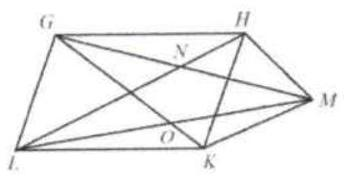
\includegraphics[width=\textwidth]{images/044(2).jpg}

\section*{Solution}
Method 1:\\
\(\angle 1=\angle 2\).\\
\(\angle L T O=\angle M K O\) since \(L H / / M K\), and since \(T H M K\) is a parallelogram, \(H T=M K\). Since \(G H K L\) is a parallelogram, the diagonals bisect each other so \(H T=L T\). Therefore, \(L T=\) \(M K \Rightarrow \triangle L T O \cong \triangle M K O\) by \(A A S\), giving \(L O=M O\), so \(O\)\\
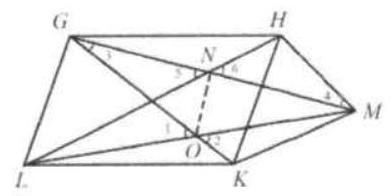
\includegraphics[width=\textwidth]{images/048(1).jpg} is the midpoint of \(L M\).


Likewise, \(\triangle N T G \cong \triangle N H M\) by AAS, since \(\angle 3=\angle 4, \angle 5=\angle 6\), and \(H M=K=\) \(G T\). Thus \(N\) is the midpoint of \(G M\).\\
Since \(N O\) is the midline of \(\triangle M G L, N O=\frac{1}{2} G L\) and \(N O / / G L\).\\
Method 2:\\
Lable the point of ntersection of \(L H\) and \(G K\) be \(T\).\\
Since \(T N / / K M\), and \(T\) is the midpoint of \(L H, N\) is the midpoint of \(G M\).\\
Since \(T O / / H M\), and \(T\) is the midpoint of \(L H, O\) is the midpoint of \(L M\).\\
Thus \(N O\) is the midline of \(\Delta M G L, N O=\frac{1}{2} G L\) and \(N O / / G L\).\\
\centering
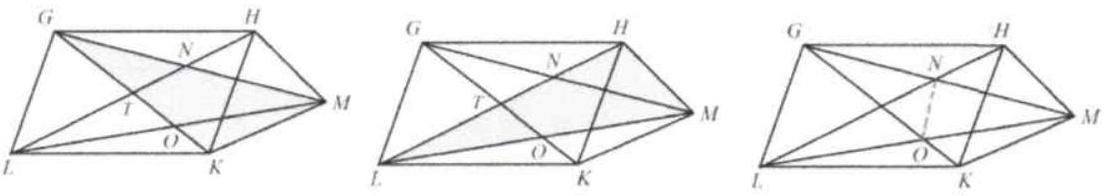
\includegraphics[width=\textwidth]{images/049(1).jpg}

\end{document}
